\documentclass[a4paper,12pt, oneside]{book}

%\usepackage{fullpage}
\usepackage[italian]{babel}
\usepackage[utf8]{inputenc}
\usepackage{amssymb}
\usepackage{amsthm}
\usepackage{graphics}
\usepackage{amsfonts}
\usepackage{amsmath}
\usepackage{amstext}
\usepackage{engrec}
\usepackage{rotating}
\usepackage{verbatim}
\usepackage[safe,extra]{tipa}
\usepackage{showkeys}
\usepackage{multirow}
\usepackage{hyperref}
\usepackage{microtype}
\usepackage{enumerate}
\usepackage{braket}
\usepackage{marginnote}
\usepackage{pgfplots}
\usepackage{cancel}
\usepackage{polynom}
\usepackage{booktabs}
\usepackage{enumitem}
\usepackage{framed}
\usepackage{pdfpages}
\usepackage{pgfplots}
\usepackage{fancyhdr}
\pagestyle{fancy}
\fancyhead[LE,RO]{\slshape \rightmark}
\fancyhead[LO,RE]{\slshape \leftmark}
\fancyfoot[C]{\thepage}


\title{Fisica}
\author{UniShare\\\\Davide Cozzi\\\href{https://t.me/dlcgold}{@dlcgold}}
\date{}

\pgfplotsset{compat=1.13}
\begin{document}
\maketitle

\definecolor{shadecolor}{gray}{0.80}

\newtheorem{teorema}{Teorema}
\newtheorem{definizione}{Definizione}
\newtheorem{esempio}{Esempio}
\newtheorem{corollario}{Corollario}
\newtheorem{lemma}{Lemma}
\newtheorem{osservazione}{Osservazione}
\newtheorem{nota}{Nota}
\tableofcontents

\renewcommand{\chaptermark}[1]{%
\markboth{\chaptername
\ \thechapter.\ #1}{}}
\renewcommand{\sectionmark}[1]{\markright{\thesection.\ #1}}

\chapter{Introduzione}
\textbf{Questi appunti sono presi a lezione. Per quanto sia stata fatta una revisione è altamente probabile (praticamente certo) che possano contenere errori, sia di stampa che di vero e proprio contenuto. Per eventuali proposte di correzione effettuare una pull request. Link: } \url{https://github.com/dlcgold/Appunti}.\\
\textbf{Grazie mille e buono studio!}

\chapter{Meccanica}
Si comincia con la Meccanica, la branca della fisica classica che studia il moto dei corpi, esprimendolo con leggi quantitative. Si ha la seguente divisione:
\begin{itemize}
\item \textbf{Cinematica}, dove si studia il moto e le sue caratteristiche indipendentemente dalle cause
\item \textbf{Dinamica}, dove si studia l'influenza delle forze nel moto 
\end{itemize}
Si utilizzano i cosiddetti \textit{punti materiali} per semplificare lo studio dei fenomeni. Un punto materiale infatti non ha estensione ma è dotato di una massa. In pratica ha dimensioni trascurabili rispetto allo spazio nel quale si muove.\\
Un altro strumento essenziale per lo studio dei fenomeni è il \textit{sistema di riferimento} mediante gli assi ortogonali:
\begin{center}
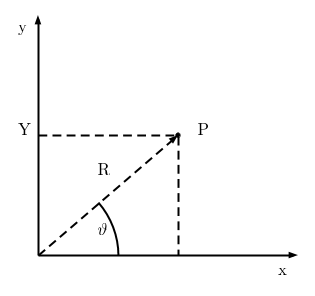
\includegraphics[scale=0.7]{img/ref.png}
\end{center}
\newpage
e si hanno le seguenti formule:
$$R=\sqrt{X^2+Y^2}$$
$$sin \vartheta=\frac{Y}{R}$$
$$cos \vartheta=\frac{X}{R}$$
$$tan \vartheta = \frac{Y}{X}$$
$$\vartheta= arctan \frac{Y}{X}$$
e per gli angoli si usano i \textit{radianti} in quanto adimensionali. L'angolo in radianti infatti è:
$$\vartheta_{rad}=\frac{Lunghezza\_arco}{raggio}$$
dove le due unità di misura esprimenti una lunghezza vengono "semplificate".\\
Si ricordano inoltre le basi del calcolo vettoriale. Tra due vettori posso fare somme e sottrazioni 
La somma non è altro che la diagonale maggiore del parallelogramma che si forma tra i due vettori. Inoltre se $\vec{A}=(a_x,a_y)$ e $\vec{B}=(b_x,b_y)$ si ha:
$$\vec{C}=\vec{A}+\vec{B}=(a_x+b_x, a_y+b_y)$$
la sottrazione è la diagonale minore e:
$$\vec{C}=\vec{A}-\vec{B}=(a_x-b_x, a_y-b_y)$$
\begin{center}
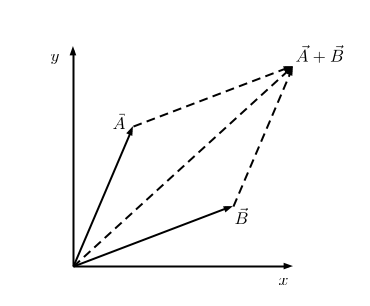
\includegraphics[scale=0.5]{img/vec.png}
\quad
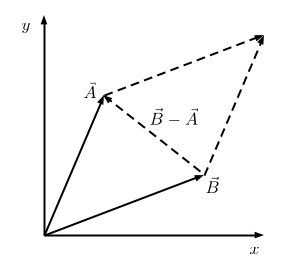
\includegraphics[scale=0.5]{img/vec2.png}
\end{center}
\section{Cinematica}
Innanzitutto qualche definizione:
\begin{itemize}
\item \textbf{Moto:} posizione in funzione del tempo in un dato sistema di riferimento
\item \textbf{Traiettoria:} luogo dei punti attraversati dal punto materiale in movimento
\item \textbf{Velocità:} variazione della posizione
\item \textbf{Accelerazione:} variazione della velocità
\item \textbf{Quiete:} assenza di movimento in un certo sistema di riferimento
\end{itemize}
Come grandezze fondamentali del movimento si hanno quindi \textit{posizione}, \textit{velocità} e \textit{accelerazione}, tutte e tre funzioni del tempo.
\subsection{Moto Rettilineo}
Rappresentando su un piano cartesiano avente la posizione come ordinata e il tempo come ascisse e rappresentando vri momenti del moto si ottiene una curva. Questa curva rappresenta la legge oraria.\\
Si ha la traiettoria più semplice, una retta. Il moto del punto quindi è esprimibile come funzione solo di $$\vec{x}(t)$$, che sarà la nostra equazione del moto.\\
Si passa quindi da un sistema di riferimento a 3 assi:
\begin{center}
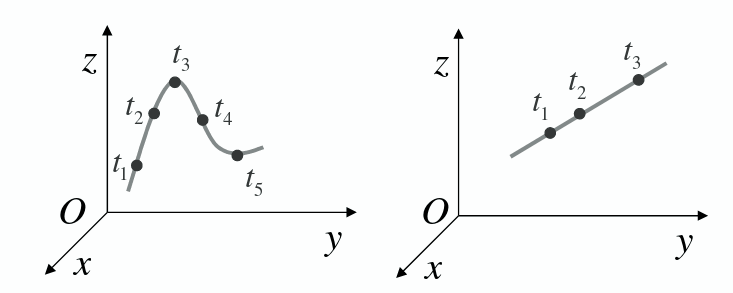
\includegraphics[scale=0.5]{img/rett.png}
\end{center}
ad uno a un asse:
\begin{center}
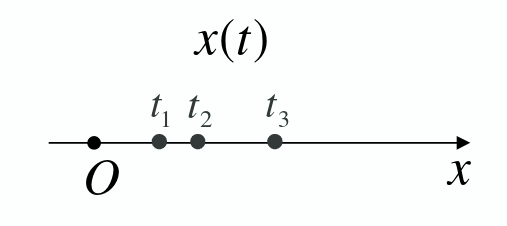
\includegraphics[scale=0.3]{img/ret2.png}
\end{center}
La scelta dell'origine della coordinata spaziale ($x=0$) e di quella temporale ($t=0$) sono arbitrari.\\
Si definisce la \textbf{distanza} come una quantità scalare la lunghezza del tratto percorso da un punto per cambiare posizione.
\subsubsection{Velocità}
Per ottenere la velocità di un punto materiale ne misuro la posizione in due diversi istanti di tempo. Si ha:
\begin{itemize}
\item \textbf{Spostamento:} $\Delta \vec{x}= x(t_2)-x(t_1)=x_2-x_1$ è un vettore che descrive la differenza di posizione tra due punti. Viene misurato in \textit{Metri (m)} secondo il Sistema Internazionale (SI). Il metro è definito come la distanza percorsa dalla luce in $\frac{1}{299792458}s$ 
\item \textbf{Intervallo di Tempo:} $\Delta t=t_2-t_1$ che viene misurato in \textit{Secondi (s)} secondo il Sistema Internazionale (SI). Il secondo è definito come la durata di $9192631770$ periodi della radiazione corrispondente alla transizione tra 2 livelli iperfini dello stato fondamentale dell'atomo di Cesio-133
\end{itemize}
Possiamo quindi definire la \textbf{Velocità Media:}
$$v_m=\frac{\Delta \vec{x}}{\Delta t}=\frac{x_2-x_1}{t_2-t_1}=\frac{\vec{v_2}-\vec{v_1}}{2}$$
Questa grandezza però non fornisce nessuna indicazione sulle caratteristiche effettive del moto. Provo a spezzare il moto in più intervalli temporali al fine di studiarne ogni variazione. Si ottiene quindi la \textbf{Velocità Istantanea}:
$$v=\lim_{\Delta t \to 0}\frac{\Delta \vec{x}}{\Delta t}=\frac{d \vec{x}(t)}{d t}$$
La velocità istantanea rappresenta la rapidità di variazione temporale della posizione nell'istante \textit{t} considerata. Il segno della velocità indica la direzione del moto sull'asse delle ascisse. La velocità è a sua volta funzione del tempo:
$$v(t)=\frac{d\vec{x}(t)}{dt}$$
che è ben rappresentata dai seguenti grafici:
\begin{center}
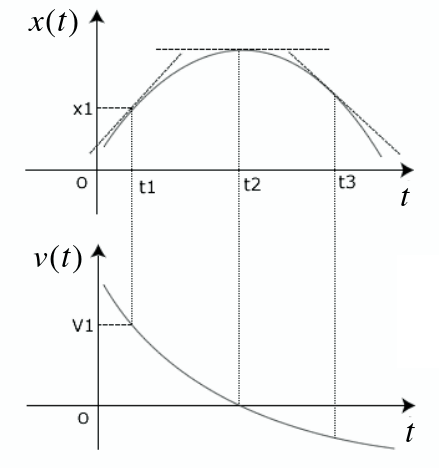
\includegraphics[scale=0.36]{img/ist.png}
\end{center}
Se \textit{v} è costante si parla di \textit{Moto Rettilineo Uniforme}. \\
Si ha quindi:
$$\Delta x = v\Delta t\to x-x_0=v(t-t_0)\to x=x_0+v(t-t_0)$$
che vale anche per $v$ non costante ma per intervalli di tempo approssimati 0, infatti tra brevi istanti di tempo si può approssimare la velocità istantanea $v(t)=\frac{dx}{dt}$ come una velocità costante. Disegniamo ora un grafico velocità tempo con la curva rappresentante la legge oraria, indicando velocità e tempo in due momenti del moto:
\begin{center}
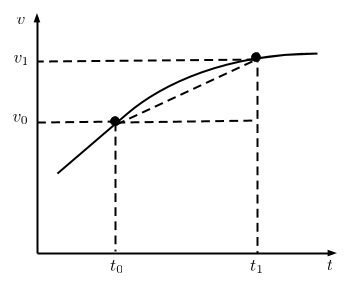
\includegraphics[scale=0.5]{img/gra.png}
\end{center}
calcolare l'area sottesa alla curva implica calcolare la differenza di posizione. Approssimo la curva ad una retta e procedo col banale calcolo del trapezio sottostante:
$$A=(t_1-t_0)(\frac{\vec{v_1}-\vec{v_0}}{2})+(t_1-t_0
)\vec{v_0}=(\frac{\vec{v_1}-\vec{v_0}}{2})\Delta t+\vec{v_0}\Delta t$$
$$A=\frac{\Delta t}{2}(\vec{v_1}-\vec{v_0}+2\vec{v_0})=\frac{\Delta t}{2}(\vec{v_0}+\vec{v_1})=\Delta t v_{med}$$
Nota quindi l'equazione del moto $$\vec{x}(t)$$ possiamo ricavare $v(t)$ derivando, infatti la posizione si ottiene, partendo dal grafico sopra, riducendo al massimo gli intervalli di tempo e calcolando la somma delle aree dei vari rettangolini .\\
Si può procedere anche al calcolo di $$\vec{x}(t)$$ avendo nota $\vec{v}(t)$. Sappiamo che lo spostamento totale è: $\Delta \vec{x}=\sum_{i=1}^n \Delta \vec{x}_i=\sum_{i=1}^n v_{m_i} \Delta t$ e che, per intervalli infinitesimi $dx=\vec{v}(t) dt$. Si ha quindi:
$$\Delta x=\underbrace{\int_{x_0}^x dx}_{\vec{x}(t)-x_0}=\int_{t_0}^t \vec{v}(t) dt$$
$$\downarrow$$
$$\vec{x}(t)=x_0+\int_{t_0}^t \vec{v}(t) dt$$
che è l'equazione del moto rettilineo per una velocità qualunque.\\
Possiamo ora anche riscrivere la forma completa della velocità media, essendo $x-x_0=\int_{t_0}^t \vec{v}(t) dt$ si ha:
$$v_m=\frac{1}{t-t_0}\int_{t_0}^t \vec{v}(t) dt$$
Possiamo analizzare ora il \textit{moto rettilineo uniforme} con \textit{v} costante. Essendo \textit{v} costante, e non più dipendente dal tempo, può essere portata fuori dall'integrale:
$$\vec{x}(t)=x_0+v\int_{t_0}^t dt=x_0+v(t-t_0)$$
che è l'equazione generale del moto rettilineo uniforme dove lo spostamento varia linearmente col tempo.\\
La velocità di esprime in metri al secondo ($\frac{m}{s}$ o \textit{m/s}) o in kilometri all'ora $\frac{km}{h}$ o \textit{km/h}). Per passare da \textit{km/h} a \textit{m/s} divido la grandezza in \textit{km/h} per 3,6, per passare da \textit{m/s} a \textit{km/h} moltiplico la grandezza in \textit{m/s} per 3,6. 
\subsubsection{Accelerazione}
Si ha che in due istanti di tempo diversi abbiamo due diverse velocità: $\vec{v}(t_1)=\vec{v_1}$ e $\vec{v}(t_2)=\vec{v_2}$. Si definisce l'\textbf{Accelerazione Media:}
$$a_m=\frac{\vec{v_2}-\vec{v_1}}{t_2-t_1}=\frac{\Delta v}{\Delta t}$$
Procediamo come per la velocità, con un grafico accelerazione-tempo e la legge del moto, calcolando l'area sottostante ottengo la differenza di posizione. Si ha una situazione più semplice ancora perché avendo $a$ costante (e quindi $ \overline{a}(t)=a_{med}=\frac{\Delta v}{\Delta t}$ e quindi $v_1=v_0+a(t_1-t_0)$) essa può essere rappresentata come una retta l'area sottostante, che questa volta è letteralmente un trapezio senza approssimazioni, è lo spostamento.
\begin{center}
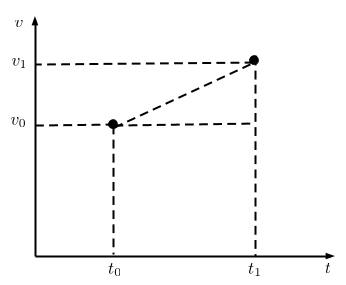
\includegraphics[scale=0.5]{img/gra2.png}
\end{center}
ovvero:
$$A=x-x_0=t_1-v_0+\frac{t_1(v_1-v_0)}{2}=t_1\frac{v_1+v_0}{2}$$ 
e quindi 
$$v_1=v_0+at_1$$
unendo con $v_1=v_0+a(t_1-t_0)$ si ottiene:
$$x-x_0=\frac{t_1}{2}(v_0+at_1+v_0)=\frac{t_1}{2}(2v_0+at_1)=v_0t_1+\frac{a}{2}t_1^2$$
$$\downarrow$$
$$x=x_0+v_0t_1+\frac{a}{2}t_1^2$$
Ora, come per la velocità, analizziamo intervalli di tempo infinitesimi ricordando che anche l'accelerazione è una funzione del tempo:
$$a(t)=\frac{dv}{dt}=\frac{d}{dt}\left(\frac{dx}{dt}\right)=\frac{d^2x}{dt^2}$$
ovvero la derivata seconda della posizione rispetto al tempo e si ha che:
\begin{itemize}
\item $a=0$ implica un moto rettilineo uniforme (si deriva una costante, \textit{v}, e si ottiene 0)
\item $a>0$ implica una velocità crescente
\item $a<0$ implica una velocità decrescente
\end{itemize}
\begin{shaded}
Proviamo ora a risalire a $\vec{v}(t)$ conoscendo \textit{a(t)}. Sappiamo che $a=\frac{dv}{dt}\rightarrow dv=a(t) dt$. Risolviamo quindi l'equazione differenziale :
$$\int_{\vec{v_0}}^v dv = \int_{t_0}^t a(t) dt\rightarrow \vec{v}(t)=\vec{v_0}+\int_{t_0}^t a(t) dt$$
che è l'equazione generale per la velocità, dove, nel caso di $a\neq 0$, ovvero di accelerazione costante, si ha:
$$\vec{v}(t)=\vec{v_0}+a\int_{t_0}^t dt=\vec{v_0}+a (t-t_0)$$
dove si nota come la velocità sia una funzione lineare del tempo se $t_0=0$, ottenendo $\vec{v}(t)=\vec{v_0}+a t$.
\end{shaded}
Cerchiamo ora l'equazione del moto in caso di\textit{ moto rettilineo uniformemente accelerato}.
si ha che: 
$$\vec{x}(t)=x_0+\int_{t_0}^t \vec{v}(t) dt= x_0+\int_{t_0}^t [\vec{v_0}+a (t-t_0)] dt$$
$$\downarrow$$
$$\vec{x}(t)=x_0+\int_{t_0}^t \vec{v_0} dt +\int_{t_0}^t a (t-t_0) dt$$
\begin{center}
\textit{porto fuori le due costanti, }$\vec{v_0}\,\, e\,\, a$
$$\downarrow$$
$$\vec{x}(t)=x_0+\vec{v_0} \int_{t_0}^t dt +a \int_{t_0}^t (t-t_0) dt$$
$$\downarrow$$
$$\vec{x}(t)=x_0+\vec{v_0} (t-t_0)+\frac{1}{2} a  (t-t_0)^2$$
dove, se si ha $t_0=0$, si ottiene:
$$\vec{x}(t)=x_0+\vec{v_0} (t-t_0)+\frac{1}{2} a  t^2$$
\end{center}
Si ha che $\overline{x}(t)$ con accelerazione costante è una parabola.\\
Ricapitolando si ha.
\begin{itemize}
\item $v=v_0+at$
\item $x=x_0+vt+\frac{1}{2}at^2$
\end{itemize}
Possiamo usare le due formule combinandole. Per esempio dalla prima prendo $$t=\frac{v-v_0}{a}$$ e lo metto nella seconda formula:
$$x=x_0+v\frac{v-v_0}{a}+\frac{1}{2}a \left(\frac{v-v_0}{a}\right)^2=x_0+\frac{v_0}{a}(v-v_0)+\frac{1}{2a}(v-v_0)^2$$
$$=x_0+\frac{1}{a}(v_0v-v_0^2+\frac{1}{2a}(v^2+v_0^2-2vv_0)=x_0+\frac{1}{2a}(2v_0v-2v_0^2+v^2+v_0^2-2v_0v)$$
$$x=x_0+\frac{v^2-v_0^2}{2a}\to v^2-v_0^2=2a(x-x_0)$$
Si nota come sia il termine $a t$ nel caso di $\vec{v}(t)$ che il termine $\frac{1}{2} a  t^2$ nel caso di $a(t)$ non dipendono dalle condizioni iniziali.\\
L'accelerazione si esprime in metri al secondo quadrato ($\frac{m}{s^2}$, $m/s^2$ o $ms^-2$)
\begin{comment}
\subsection{Moto Verticale}
Sperimentale si scopre come un qualunque corpo lasciato libero di cadere nei pressi della superficie terrestre si muove verso il basso con un'accelerazione costante $g\simeq 9.81\, ms^{-2}$ (si trascurano attrito dell'aria e si trattano piccole altitudini). Il valore di \textit{g} non è costante in ogni parte del mondo ma può variare fino a circa il $0.6\%$.\\
Impostiamo un sistema di riferimento con l'asse \textit{x} crescente verso l'alto e quindi con $a=-g=-9.81 ms^{-2}$. Si avrà un corpo in caduta libera da un'altezza \textit{h}:
\begin{center}
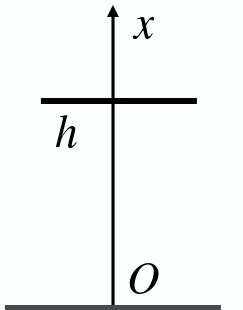
\includegraphics[scale=0.3]{img/vert.png}
\end{center}
Si hanno le seguenti condizioni iniziali:
\begin{itemize}
\item $t=t_0=0$
\item $x_0=h$
\item $\vec{v_0}=0$
\end{itemize}
Con queste premesse otteniamo:
\begin{itemize}
\item \textbf{Equazione del moto:}
$$\vec{x}(t)=x_0+\vec{v_0} t+\frac{1}{2} a  t^2$$
$$\downarrow$$
$$\vec{x}(t)=h-\frac{1}{2} g t^2$$
\item \textbf{Equazione della velocità:}
$$\vec{v}(t)=\vec{v_0}+a t$$
$$\downarrow$$
$$\vec{v}(t)=-g t$$
\end{itemize}
Posso quindi ottenere il tempo di caduta, ponendo $x=0$ nell'equazione del moto:
$$h-\frac{1}{2} g t^2=0\rightarrow t_c=\sqrt{\frac{2 h}{g}}$$
e posso ottenere la velocità al suolo:
$$v_c=v(t_c)=-g t_c=-g \sqrt{\frac{2 h}{g}}=-\sqrt{2 g h}$$
Imponiamo ora una velocità iniziale $-\vec{v_1}$, quindi verso il basso:
\begin{center}
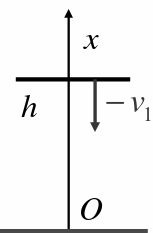
\includegraphics[scale=0.4]{img/vert2.png}
\end{center} 
Si hanno le seguenti condizioni iniziali:
\begin{itemize}
\item $t=t_0=0$
\item $x_0=h$
\item $\vec{v_0}=-\vec{v_1}$
\end{itemize}
\begin{itemize}
\item \textbf{Equazione del moto:}
$$\vec{x}(t)=x_0+\vec{v_0} t+\frac{1}{2} a  t^2$$
$$\downarrow$$
$$\vec{x}(t)=h-\vec{v_1}t-\frac{1}{2} g t^2$$
\item \textbf{Equazione della velocità:}
$$\vec{v}(t)=\vec{v_0}+a t$$
$$\downarrow$$
$$\vec{v}(t)=-\vec{v_1}-gt$$
\end{itemize}
Posso quindi ottenere il tempo di caduta, ponendo $x=0$ nell'equazione del moto:
$$h-\vec{v_1}t-\frac{1}{2} g t^2=0-\rightarrow \frac{1}{2} g t^2 +\vec{v_1}t-h=0$$
$$\downarrow$$
$$t_c=\frac{-\vec{v_1}\pm \sqrt{\vec{v_1}^2+2gh}}{g}$$
\begin{center}
\textit{ma $t<0$ non è una soluzione fisica, quindi tengo solo la soluzione col +}
\end{center}
$$t_c=-\frac{\vec{v_1}}{g}+\frac{1}{g}\sqrt{\vec{v_1}^2+2gh}$$
e posso ottenere la velocità al suolo:
$$v_c=-\vec{v_1}-gt_c=-\vec{v_1}-g\left[-\frac{\vec{v_1}}{g}+\frac{1}{g}\sqrt{\vec{v_1}^2+2gh}\right]=-\sqrt{\vec{v_1}^2+2gh}$$
Con una velocità iniziale verso il basso avremo un tempo di caduta inferiore e una velocità al suolo maggiore rispetto alla partenza da fermo.\\
Analizziamo ora il moto verticale di un punto materiale lanciato dal basso verso l'alto con velocità $\vec{v_2}$:
\begin{center}
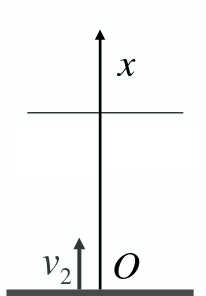
\includegraphics[scale=0.4]{img/vert3.png}
\end{center}
Si hanno le seguenti condizioni iniziali:
\begin{itemize}
\item $t=t_0=0$
\item $x_0=0$
\item $\vec{v_0}=\vec{v_2}$
\end{itemize}
\begin{itemize}
\item \textbf{Equazione del moto:}
$$\vec{x}(t)=x_0+\vec{v_0} t+\frac{1}{2} a  t^2$$
$$\downarrow$$
$$\vec{x}(t)=\vec{v_2}t-\frac{1}{2} g t^2$$
\item \textbf{Equazione della velocità:}
$$\vec{v}(t)=\vec{v_0}+a t$$
$$\downarrow$$
$$\vec{v}(t)=\vec{v_2}-gt$$
\end{itemize}
Inizialmente si ha $v>0$, finché il punto sale verso l'alto, fino a fermarsi. Con $v=0$ si ha l'altezza massima. Si ha quindi:
$$v=\vec{v_2}-gt=0\rightarrow t_{max}=\frac{\vec{v_2}}{g}$$
e quindi:
$$x_{max}=x(t_{max})=\vec{v_2}\frac{\vec{v_2}}{g}-\frac{1}{2}g\frac{\vec{v_2}^2}{g^2}=\frac{1}{2}\frac{\vec{v_2}^2}{g}$$
raddoppiando la velocità iniziale avrò quindi un'altezza 4 volte superiore. Da questp momento in poi di avrà la caduta libera da $h=x-max$ con $\vec{v_0}=0$:
$$t_c=\sqrt{\frac{2h}{g}}=\sqrt{\frac{2x_{max}}{g}}=\sqrt{\frac{2}{g}\left(\frac{1}{2}\frac{\vec{v_2}^2}{g}\right)}=\frac{\vec{v_2}}{g}$$
e quindi si avrà:
$$t_{tot}=t_{max}+t_c=\frac{2\vec{v_2}}{g}$$
\subsection{Moto Armonico}
Si ha la seguente equazione del moto per un \textit{moto armonico semplice} lungo un asse rettilineo:
$$\vec{x}(t)=Asin(\omega t+\varphi)$$
con:
\begin{itemize}
\item \textit{A} ampiezza, espressa in $m$ e costante
\item $\omega$ pulsazione, espressa in $s^{-1}$ e costante
\item $\varphi$ fase iniziale
\item $\omega t+\varphi$ è detta fase
\end{itemize}
Si ha inoltre:
\begin{itemize}
\item $sin(\omega t+\varphi)$ che è la traiettoria e si ha che $-1\geq sin(\omega t+\varphi)\leq 1$
\item $x_0=x(0)=asin\varphi$ è la posizione iniziale generica
\end{itemize}
$\vec{x}(t)=Asin(\omega t+\varphi)$ è una funzione periodica con periodo $T=2\pi$ (la posizione si ripete dopo ogni periodo \textit{T}). Consideriamo $T=t_2-t_1=2\pi$. Si ha quindi che:
$$x(t_2)=x(t_1)$$
$$\downarrow$$
$$Asin(\omega t_2+\varphi)=Asin(\omega t_1+\varphi)$$
$$\downarrow$$
$$(\omega t_2+\varphi)-(\omega t_1+\varphi)=2\pi$$
$$\downarrow$$
$$\omega(t_2-t_1)=2\pi$$
$$\downarrow$$
$$T=\frac{2\pi}{\omega}$$
Si ha quindi che:
\begin{itemize}
\item $\omega=\frac{2\pi}{T}$, la pulsazione è inversamente proporzionale al periodo
\item \textbf{Frequenza:} $\nu =\frac{1}{T}$ quindi $\omega=2\pi\ni$
\end{itemize}
Pulsazione e frequenza sono indipendenti dall'ampiezza.\\
Posso ora trovare velocità ed accelerazione dall'equazione del \\moto $\vec{x}(t)=Asin(\omega t+\varphi)$:
\begin{itemize}
\item \textbf{velocità:} $\vec{v}(t)=\frac{d\vec{x}(t)}{dt}=A\omega\, cos(\omega t+\varphi)$
\item \textbf{accelerazione:} $\vec{v}(t)=\frac{d\vec{v}(t)}{dt}=\frac{d^2\vec{x}(t)}{dt^2}=-A\omega^2 \,sin(\omega t+\varphi)=-\omega^2 \vec{x}(t)$
\end{itemize}
Ampiezza di $\vec{v}(t)$ e \textit{a(t)} dipendono dalla pulsazione. Le tre curve \textit{$\vec{x}(t)$}, $\vec{v}(t)$ e \textit{a(t)} hanno lo stesso andamento ma sono sfasate tra loro. Ricordando che $sin(\alpha+\frac{\pi}{2}=cos \alpha$ e che $sin(\alpha+\pi)=-sin\alpha$ notiamo che $\vec{v}(t)$ è sfasata di $\frac{\pi}{2}$ rispetto a \textit{$\vec{x}(t)$} (\textit{quadratura di fase}) e che \textit{a(t)} è sfasata di $\pi$ rispetto a \textit{$\vec{x}(t)$} (\textit{opposizione di fase}) 
\begin{center}
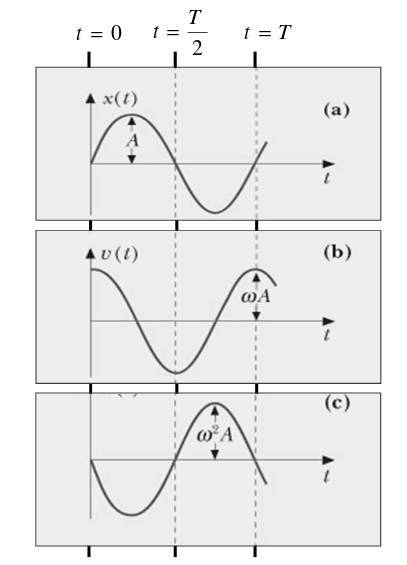
\includegraphics[scale=0.5]{img/arm.png}
\end{center}
\subsection{Moto nel Piano}
Si passa ora al moto in 2 dimensioni quindi con una traiettoria curva (e non più una retta).\\
Si introducono le coordinate cartesiane ($$\vec{x}(t)$$ e $y(t)$) e quelle polari ($r(t)$ e $\vartheta(t)$). Si hanno le seguenti formule per il passaggio da coordinate cartesiane a polari:
$$r=\sqrt{x^2+y^2}$$
$$tan\,\vartheta=\frac{y}{x}$$
e le seguenti per il passaggio da coordinate polari a cartesiane:
$$x=r\,cos\,\vartheta$$
$$y=r\,sin\,\vartheta$$
\begin{center}
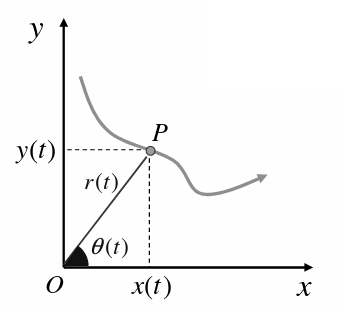
\includegraphics[scale=0.4]{img/pia.png}
\end{center}
Il moto di $P$ è descritto attraverso l'evoluzione del vettore posizione:
$$\vec{r}(t)\equiv (\vec{x}(t),y(t))$$
Si introducono inoltre i versori degli assi $\vec{u}_x,\,\vec{u}_y$, ricordando che $|\vec{u}_x|=|\vec{u}_y|=1$ e che i versori restano fissi nel tempo. Si ottiene quindi:
$$\vec{r}(t)=\vec{x}(t)\vec{u}_x+y(t)\vec{u}_y$$
\begin{center}
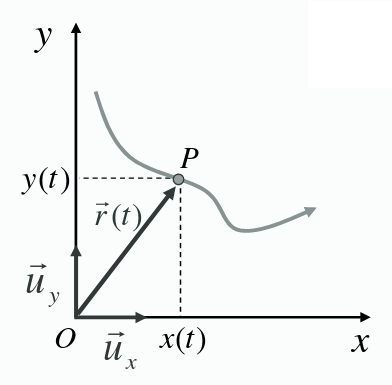
\includegraphics[scale=0.4]{img/pia2.png}
\end{center}
\newpage
Suppongo ora la traiettoria fissata e nota a priori. Fissata un'origine $O$, una posizione $s(t)$ e la velocità $v=\frac{ds}{dt}$ si ha che il moto è completamente determinato. Si ha una generalizzazione del moto rettilineo su una traiettoria curva.\\
Prendiamo ora in considerazione il seguente caso:
\begin{center}
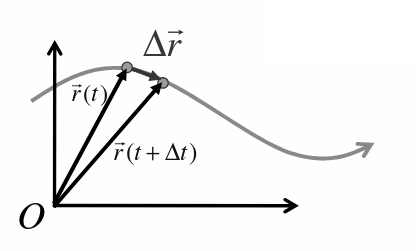
\includegraphics[scale=0.4]{img/pia3.png}
\end{center}
si ha il vettore spostamento:
$$\Delta\vec{r}(t)=\vec{r}(t+\Delta t)-\vec{r}(t)$$
e il vettore velocità media:
$$\vec{v}_m\equiv\frac{\Delta\vec{r}}{\Delta t}$$
e il vettore velocità istantanea:
$$\vec{v}(t)=\lim_{\Delta t\to 0}\frac{\Delta\vec{r}}{\Delta t}=\lim_{\Delta t\to 0}\frac{\vec{r}(t+\Delta t)-\vec{r}(t)}{\Delta t}=\frac{d\vec{r}}{dt}$$
al limite $\Delta t\to 0$ lo spostamento infinitesimo si dispone sulla tangente alla traiettoria nel punto $P$: 
$$d\vec{r}=ds\vec{u}_T$$
con $|\vec{u}_T|=1$ versore della tangente che indica una direzione variabile nel tempo. Per il vettore velocità avremo:
$$\vec{v}=\frac{d\vec{r}}{dt}=\frac{ds}{dt}\vec{u}_T=v\vec{u}_T$$
con $v$ indicate il modulo della velocità e $\vec{u}_T$ la direzione.
\newpage
 Quanto appena descritto è visualizzabile nelle seguenti immagini:
\begin{center}
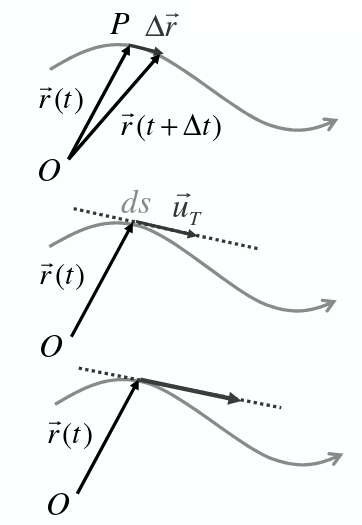
\includegraphics[scale=0.4]{img/pia4.png}
\end{center}
Analizziamo ora meglio la velocità nelle componenti cartesiane. Essendo $\vec{v}_m=\frac{\Delta\vec{r}}{\Delta t}$ e $\vec{r}(t)=\vec{u}_x+y(t)\vec{u}_y$ si ottiene:
$$\vec{v}=\frac{dx}{dt}\vec{u}_x+\frac{dy}{dt}\vec{u}_y=v_x\vec{u}_x+v_y\vec{u}_y$$
con il modulo della velocità:
$$v=|\vec{v}|=\sqrt{v_x^2+v_y^2}$$
Ecco un'immagine di quanto detto:
\begin{center}
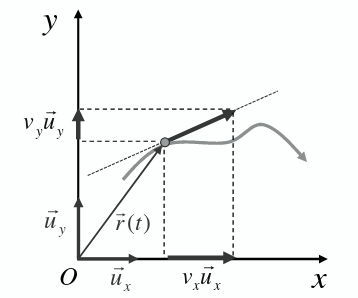
\includegraphics[scale=0.6]{img/pia5.png}
\end{center}
\newpage
Passiamo alle componenti polari. Essendo $\vec{v}_m=\frac{\Delta\vec{r}}{\Delta t}$ e $\vec{r}(t)=r(t)\vec{u}_r(t)$ (col versore $\vec{u}_r$ mostrato in figura) si ottiene:
$$\vec{v}=\frac{d}{dt}(r\vec{u}_r)=\frac{dr}{dt}\vec{u}_r+r\frac{d\vec{u}_r}{dt}=\frac{dr}{dt} \vec{u}_r+r\frac{d\vartheta}{dr}\vec{u}_\vartheta$$
in quanto solitamente la derivata di un versore è: 
$$\frac{d\vec{u}}{dt}=\frac{\vec{u}(t+dt)-\vec{u}(t)}{dt}=\frac{d\vartheta}{dt}\vec{u}_\bot$$
Ecco un'immagine di quanto detto:
\begin{center}
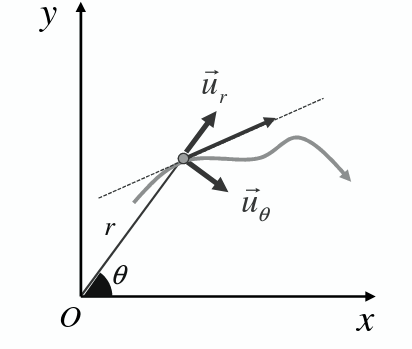
\includegraphics[scale=0.5]{img/pia6.png}
\end{center}
Possiamo approfondire ancora lo studio della velocità in componenti polari infatti:
$$\vec{v}=\underbrace{\frac{dr}{dt} \vec{u}_r}_{\vec{v_r}}+\underbrace{r\frac{d\vartheta}{dr}\vec{u}_\vartheta}_{\vec{v}_\vartheta}$$
con:
\begin{itemize}
\item $\vec{v_r}$ è la \textbf{velocità radiale} e $|\vec{v_r}|=\frac{dr}{dt}$  è la variazione di $r$
\item $\vec{v_\vartheta}$ è la \textbf{velocità traversa} e $|\vec{v_\vartheta}|=r\frac{d\vartheta}{dt}$ è la variazione della direzione
\end{itemize}
quindi:
$$\vec{v}=\vec{v_r}+\vec{v_\vartheta}$$
e quindi:
$$|\vec{v}|=\sqrt{v_r^2+v_\vartheta^2}=\sqrt{\left(\frac{dr}{dt}\right)^2+r^2\left(\frac{d\vartheta}{dt}\right)^2}$$
\newpage
Ecco un'immagine che spiega quanto detto:
\begin{center}
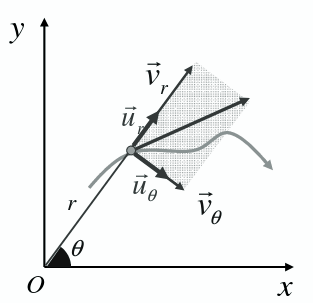
\includegraphics[scale=0.5]{img/pia7.png}
\end{center}
Passiamo ora all'accelerazione nel piano. Essa è, come sappiamo, la variazione della velocità $\vec{v}=v\vec{u}_T$ ma, se nel moto rettilineo è solo la variazione del modulo, nel moto del piano si ha anche la variazione della direzione. Iniziamo sapendo che $\vec{a}=\frac{d\vec{v}}{dt}$. Quindi:
$$\vec{a}=\frac{d}{dt}(v\vec{u}_t)=\frac{dv}{dt}\vec{u}_T+v\frac{d\vec{u}_t}{dt}$$
ricordando la derivata di un versore si ottiene:
$$\vec{a}=\frac{dv}{dt}\vec{u}_T+v\frac{d\phi}{dt}\vec{u}_N$$
con:
\begin{itemize}
\item $\vec{u}_N$ versore perpendicolare al versore tangente
\item $\frac{dv}{dt}\vec{u}_T$ variazione del modulo velocità, detta $\vec{a}_T$ \textbf{accelerazione tangenziale}
\item $v\frac{d\phi}{dt}\vec{u}_N$ variazione della direzione, detta $\vec{a}_T$ \textbf{accelerazione normale o centripeta}
\end{itemize}
quindi:
$$\vec{a}=\vec{a}_T+\vec{a}_N$$
procedendo con l'analisi della traiettoria si nota come essa possa essere approssimata da una circonferenza con un certo raggio $R$ che può essere usato come raggio di curvatura. Si ha quindi $ds=R\,d\phi$ e quindi:
$$\frac{d\,\phi}{dt}=\frac{1}{R}\frac{ds}{dt}=\frac{1}{R}v$$
Posso quindi sostituire $\frac{d\,\phi}{dt}$ nella formula precedentemente trovata dell'accelerazione ottenendo:
$$\vec{a}=\frac{dv}{dt}\vec{u}_T+\frac{v^2}{R}\vec{u}_N$$
quindi $\vec{a}_N$ può anche essere indicata con $\vec{a}_N=\frac{v^2}{R}\vec{u}_N$. Da questi ultimi due risultati si intuiscono due cose:
\begin{enumerate}
\item se $r\to\infty$ si ha $\vec{a}_N=0$ e quindi un moto rettilineo
\item se $\frac{dv}{dt}=0$ si ha $\vec{a}_T=0$ e quindi un moto curvilineo uniforme con solo il cambiamento della direzione
\end{enumerate}
Si ha infine il modulo dell'accelerazione:
$$a=|\vec{a}|=\sqrt{\left(\frac{dv}{dt}\right)^2+\frac{v^4}{R^2}}$$
Ecco un'immagine di quanto detto:
\begin{center}
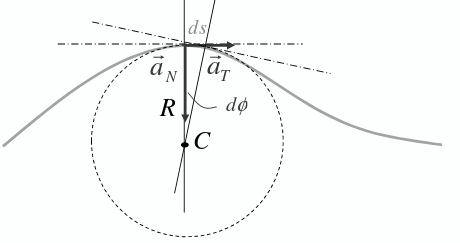
\includegraphics[scale=0.5]{img/pia8.png}
\end{center}
Proiettiamo ora l'accelerazione sugli assi del sistema cartesiano:
$$\vec{a}=\frac{dv_x}{dt}\vec{u}_x+\frac{dv_y}{dt}\vec{u}_y=a_x\vec{u}_x+a_y\vec{u}_y$$
analizziamo anche quanto succede sul piano:
\begin{center}
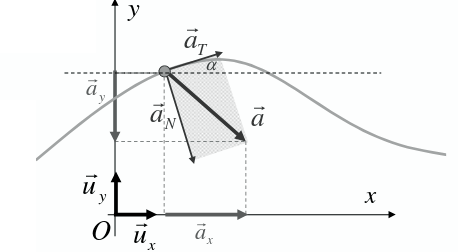
\includegraphics[scale=0.6]{img/pia9.png}
\end{center}
Possiamo ora scrivere le componenti cartesiane in funzione di quella tangenziale e di quella centripeta:
\begin{itemize}
\item per l'ascisse:
$$a_x=(a_T)_x+(a_N)_x=a_tcos\,\alpha+a_ncos\left(\frac{\pi}{2}-\alpha\right)=\frac{dv}{dt}cos\,\alpha+\frac{v^2}{R}sin\,\alpha$$
\item per l'ordinata:
$$a_y=\frac{dv}{dt}sin\,\alpha-\frac{v^2}{R}cos\,\alpha$$
\end{itemize}
\subsection{Moto Circolare}
Si tratta di un caso particolare di moto curvilineo nel piano. In generale si ha il modulo della velocità non uniforme. Si hanno quindi:
\begin{itemize}
\item \textit{coordinate polari}:
\begin{itemize}
\item angolo $\theta(t)$
\item raggio $r(t)=R=costante$
\end{itemize}
\item \textit{coordinate curvilinee}:
\begin{itemize}
\item posizione misurata lungo la traiettoria $s(t)=R\theta (t)$
\end{itemize}
\item \textit{coordinate cartesiane:}
\begin{itemize}
\item $\vec{x}(t)=R\,cos\,\theta(t)$
\item $y(t)=R\,sin\,\theta(t)$
\end{itemize}
\end{itemize}
ovvero:
\begin{center}
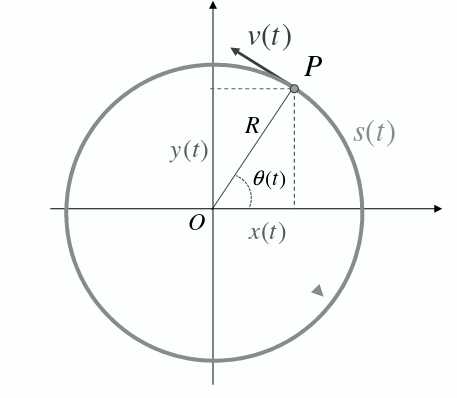
\includegraphics[scale=0.52]{img/cir.png}
\end{center}
Iniziamo ad analizzare il moto circolare. Considero il punto $P$ in due istanti $t$ e $t+\Delta t$. Quindi avrò $\theta (t)=\theta_1$ e $\theta(t+\Delta t)=\theta_2$. Nel complesso si ha $\Delta \theta= \theta_2-\theta_1$:
\begin{center}
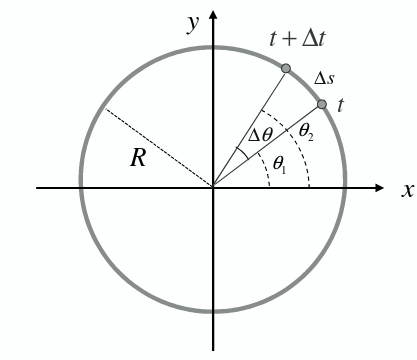
\includegraphics[scale=0.52]{img/cir2.png}
\end{center}
Si definisce innanzitutto la velocità angolare media:
$$\omega_m=\frac{\Delta\theta}{dt}$$
mentre per la velocità angolare istantanea si ha:
$$\omega=\lim_{\Delta t\to 0}\frac{\Delta\theta}{dt}=\frac{d\theta}{dt}$$
Si indica ora la velocità angolare in funzione di $v$ e $R$, ricordando che $ds=Rd\theta$:
$$\omega=\frac{d\theta}{dt}=\frac{1}{R}\frac{ds}{dt}=\frac{v}{R}$$
quindi la velocità angolare è proporzionale al modulo della velocità ed inversamente proporzionale al raggio. Inoltre $v=\omega R$. Partiamo da qui per approfondire la velocità nel moto circolare. Sappiamo che in generale nel moto curvilineo si ha: $\vec{v}=\frac{dr}{dt}\vec{u_r}+r\frac{d\theta}{dt}\vec{u_\theta}$. Si ha che $\frac{dr}{dt}=0$ quindi:
$$\vec{v}=R\frac{d\theta}{dr}\vec{u}_\theta=R\omega\vec{u}_\theta$$
\newpage
in quanto $R$ è costante e quindi si ha come modulo della velocità:
$$\vec{v}(t)=|\vec{v}(t)|=\omega(t)R$$
graficamente si ha:
\begin{center}
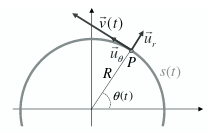
\includegraphics[scale=0.9]{img/cir3.png}
\end{center}
Si ha inoltre che se si parla di moto circolare uniforme si ha che $v=\omega R$ è costante in quanto $\omega$ è costante.\\
Passiamo all'accelerazione nel moto circolare uniforme. Si ha solo l'accelerazione centripeta in quanto $\frac{dv}{dt}=0$
$$\vec{a}=\frac{v^2}{R}\vec{U}_N$$
con $v^2$ costante e si ha il modulo dell'accelerazione pari a:
$$a=|\vec{a}|=\frac{v^2}{R}=\frac{(\omega R)^2}{R}=\omega^2 R=\omega \, v$$
Quindi per il moto lungo la traiettoria si ha:
\begin{itemize}
\item $s(t)=s_0+vt$
\item $\theta(t)=\theta_0+\omega t$
\end{itemize}
e nel moto circolare uniforme si può notare un moto periodico con periodo:
$$T=\frac{2\pi R}{v}=\frac{2\pi R}{\omega R}=\frac{2\pi}{\omega}$$
vediamo ora l'accelerazione in caso di moto non uniforme, quindi con $\vec{a}=\vec{a}_T+\vec{a}_N$ e con $\vec{v}(t)=\omega(t)R$. Definisco un'accelerazione angolare media:
$$\alpha_m=\frac{\omega_2-\omega_1}{\Delta t}=\frac{\Delta\omega}{\Delta t}$$
e l'accelerazione angolare istantanea, si ricorda che $\omega=\frac{v}{r}$:
$$\alpha=\lim_{\Delta t\to 0}\frac{\Delta\omega}{\Delta t}=\frac{d\omega}{dt}=\frac{1}{R}\frac{dv}{dt}=\frac{1}{R}a_T$$
\newpage
visivamente:
\begin{center}
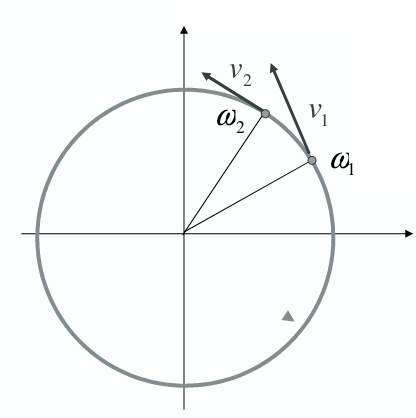
\includegraphics[scale=0.4]{img/cir4.png}
\end{center}
Possiamo quindi riscrivere accelerazione normale e tangenziale in funzione di quantità angolari:
\begin{itemize}
\item $a_N=\frac{v^2}{R}\xrightarrow{v=\omega R} a_N=\omega^2 R$
\item $a_T=\frac{dv}{dt}\xrightarrow{v=\omega R} a_T=\frac{d\omega}{dt}R=\alpha R$
\end{itemize}
quindi:
$$\vec{a}=\alpha R\vec{u}_T+\omega^2 R\vec{u}_N= R(\alpha \vec{u}_T+\omega^2 \vec{u}_N)$$
quindi infine:
\begin{itemize}
\item $\omega(t)=\omega_0+\int_{t_0}^t \alpha dt=\omega_0+\alpha \int_{t_0}^t dt=\omega_0+\alpha t$ in quanto $t_0=0$
\item $\theta(t)=\theta_0+\int_{t_0}^t \omega (t)dt=\theta_0+\int_{t_0}^t (\omega_0+\alpha t)dt=\theta_0+\omega_0t+\frac{1}{2}\alpha t^2$, dove si nota l'analogia con l'accelerazione nel moto rettilineo
\item $a_N=\omega^2 R=(\omega_0+\alpha t)^2 R$
\end{itemize}
Diamo nuovamente un'occhiata alla velocità angolare $\omega=\frac{d\theta}{dt}=\frac{v}{R}$. Si ha che è una quantità scalare. Studiamo ora la notazione vettoriale di $\vec{\omega}$. Questo vettore ha direzione ortogonale alla circonferenza e , visto dalla punta di $\vec{\omega}$ il moto appare antiorario. SI ha quindi che $\vec{\omega}\times \vec{r}=\vec{v}$ e:
$$|\vec{v}|=\omega Rsin\,\frac{\pi}{2}=\omega R$$
anche se il vettore $\vec{\omega}$si può applicare a qualunque punto dell'asse $z$, ottenendo:
$$|\vec{v}|=\omega Rsin\,\phi=\omega R$$
\newpage
graficamente si ha a sinistra il caso con applicazione sull'origine normale e a destra il caso applicazione in un punto a scelta:
\begin{center}
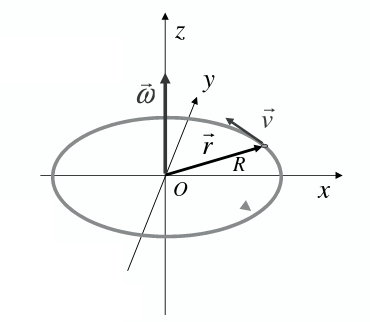
\includegraphics[scale=0.5]{img/cir5.png}
\quad
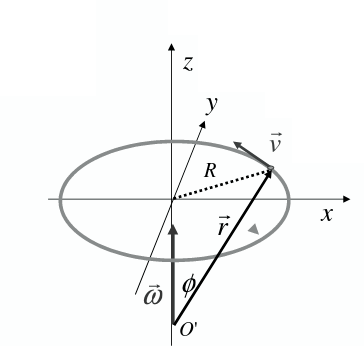
\includegraphics[scale=0.5]{img/cir6.png}
\end{center}
%vedere se serve moto nei pressi della superficie terrestre, moto parabolico!
%\section{Dinamica}
\end{comment}
\end{document}